\documentclass[aspectratio=169]{beamer}
\usetheme{metropolis}
\usepackage[T1]{fontenc}
\usepackage{lmodern}
\usepackage{tikz}
\usepackage{fontawesome5}
\usetikzlibrary{arrows.meta, positioning, shapes.geometric}

\title{Raf's Perspective on Matrix Games}
\subtitle{and a desire to improve decision making by playing matrix games with LLMs \faGamepad}
\author{Rafael}
\date{2025}
\institute{\scriptsize * Generative AI has been used in the creation of this presentation 
\\ * Rafael is a hobbyist and has never seen a matrix game played by humans}

\setbeamercolor{background canvas}{bg=black!5}
\setbeamertemplate{frame footer}{\insertshortauthor}

\begin{document}

\maketitle
\note{ 
  I have been working on getting llms to play matrix games for the last month or so
  I was Inspired by the NSDMG
}

% ============================================================
\begin{frame}{The Scenario}
  \centering
  \LARGE
  \textbf{You're a rebel commander in Syria.}

  \vspace{1em}
  \large
  Chemical weapons are missing. \\
  Putin is on the phone. \\
  The UN is watching. \\

  \vspace{1em}
  \textbf{What do you do?}
\end{frame}
\note{ Get as far through a round until no longer smooth }

% ============================================================
\begin{frame}{Traditional Wargames vs Matrix Games}
  \begin{columns}[T]
    \begin{column}{0.48\textwidth}
      \textbf{Traditional Wargames:}
      \begin{itemize}
        \item Consult 200-page rulebook
        \item Check 47 modifiers
        \item Roll 3d6, cross-reference table
        \item Calculate supply chains
        \item 20 minutes later...
        \item Still on turn 1
      \end{itemize}
    \end{column}

    \begin{column}{0.48\textwidth}
      \textbf{Matrix Games:}
      \begin{itemize}
        \item \textcolor{blue}{\textbf{Declare:}} "I appeal to the UN for an investigation"
        \item \textcolor{green!60!black}{\textbf{Because:}}
          \begin{itemize}
            \item I have credibility
            \item Russia wants to avoid blame
            \item It distracts from my actual plan
          \end{itemize}
        \item Roll 2d6
      \end{itemize}
    \end{column}
  \end{columns}

  \vspace{1em}
  \centering
\end{frame}
\note{ 
  And that is the core of a matrix game. fairly straightforward
  normally it would start with some background
  and we would progress to
  Compare this to traditional games where you have large rule books and formulas to follow
}

% ============================================================
\begin{frame}{A Cherry Picked History of Wargaming and Strategizing Developments}
  \centering
  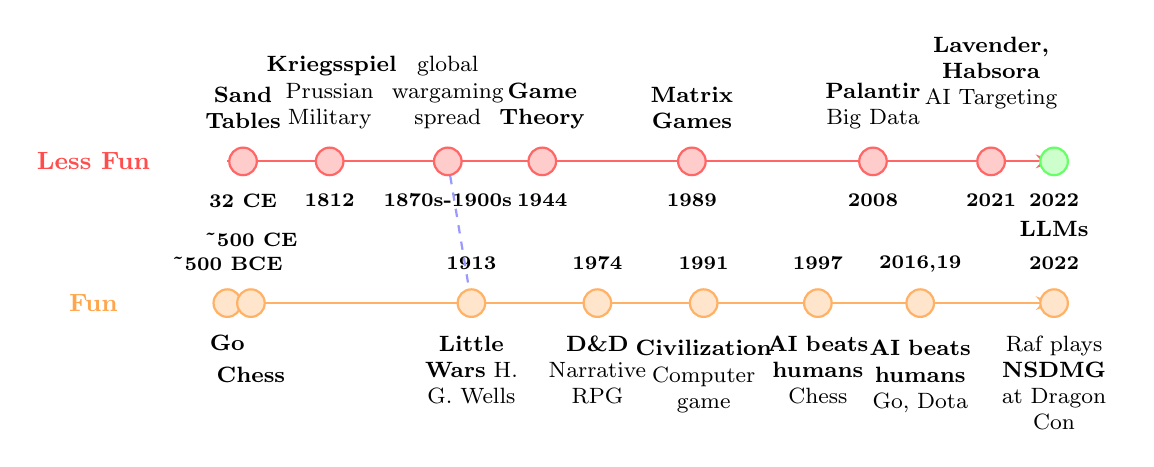
\begin{tikzpicture}[
    every node/.style={font=\footnotesize},
    trunk/.style={thick, -Stealth},
    crosspol/.style={thick, dashed, blue!40},
    serious/.style={circle, fill=red!20, draw=red!60, thick, minimum size=0.35cm},
    rec/.style={circle, fill=orange!20, draw=orange!60, thick, minimum size=0.35cm},
    ai/.style={circle, fill=green!20, draw=green!60, thick, minimum size=0.35cm},
    year/.style={font=\scriptsize\bfseries}
  ]
    % Professional/Serious timeline (top)
    \draw[trunk, red!60] (-0.5,1.8) -- (10.0,1.8);
    \node[font=\small\bfseries, red!70] at (-2.2,1.8) {Less Fun};

    \node[serious] at (-0.3,1.8) (s0) {};
    \node[year] at (-0.3,1.3) {32 CE};
    \node[text width=1.4cm, align=center, above=0.1cm of s0] {\textbf{Sand Tables}};

    \node[serious] at (0.8,1.8) (s1) {};
    \node[year] at (0.8,1.3) {1812};
    \node[text width=1.6cm, align=center, above=0.1cm of s1] {\textbf{Kriegsspiel} \\ Prussian Military};

    \node[serious] at (2.3,1.8) (s1b) {};
    \node[text width=1.6cm, align=center, above=0.1cm of s1b] {global wargaming spread};
    \node[year] at (2.3,1.3) {1870s-1900s};

    \node[serious] at (3.5,1.8) (s1c) {};
    \node[year] at (3.5,1.3) {1944};
    \node[text width=1.6cm, align=center, above=0.1cm of s1c] {\textbf{Game Theory}};

    \node[serious] at (5.4,1.8) (s2) {};
    \node[year] at (5.4,1.3) {1989};
    \node[text width=1.6cm, align=center, above=0.1cm of s2] {\textbf{Matrix Games}};

    \node[serious] at (7.7,1.8) (s3a) {};
    \node[year] at (7.7,1.3) {2008};
    \node[text width=1.8cm, align=center, above=0.1cm of s3a] {\textbf{Palantir} \\ Big Data};

    \node[serious] at (9.2,1.8) (s3b) {};
    \node[year] at (9.2,1.3) {2021};
    \node[text width=1.8cm, align=center, above=0.35cm of s3b] {\textbf{Lavender, Habsora} \\ AI Targeting};

    \node[ai] at (10,1.8) (s4) {};
    \node[year] at (10,1.3) {2022};
    \node[text width=1.6cm, align=center, below=0.45cm of s4] {\textbf{LLMs}};

    % Recreational timeline (bottom)
    \draw[trunk, orange!60] (-0.5,0) -- (10.0,0);
    \node[font=\small\bfseries, orange!70] at (-2.2,0) {Fun};

    \node[rec] at (-0.5,0) (r0a) {};
    \node[year] at (-0.5,0.5) {\textasciitilde500 BCE};
    \node[text width=1.3cm, align=center, below=0.1cm of r0a] {\textbf{Go}};

    \node[rec] at (-0.2,0) (r0b) {};
    \node[year] at (-0.2,0.8) {\textasciitilde500 CE};
    \node[text width=1.3cm, align=center, below=0.5cm of r0b] {\textbf{Chess}};

    \node[rec] at (2.6,0) (r1) {};
    \node[year] at (2.6,0.5) {1913};
    \node[text width=1.6cm, align=center, below=0.1cm of r1] {\textbf{Little Wars} H. G. Wells};

    \node[rec] at (4.2,0) (r3) {};
    \node[year] at (4.2,0.5) {1974};
    \node[text width=1.6cm, align=center, below=0.1cm of r3] {\textbf{D\&D} \\ Narrative RPG};

    \node[rec] at (5.55,0) (r5) {};
    \node[year] at (5.55,0.5) {1991};
    \node[text width=1.8cm, align=center, below=0.16cm of r5] {\textbf{Civilization} \\ Computer game};

    \node[rec] at (7.0,0) (r6) {};
    \node[year] at (7.0,0.5) {1997};
    \node[text width=1.5cm, align=center, below=0.1cm of r6] {\textbf{AI beats humans} \\ Chess};

    \node[rec] at (8.3,0) (r7) {};
    \node[year] at (8.3,0.5) {2016,19};
    \node[text width=1.5cm, align=center, below=0.16cm of r7] {\textbf{AI beats humans} \\ Go, Dota};

    \node[rec] at (10,0) (r4) {};
    \node[year] at (10,0.5) {2022};
    \node[text width=1.6cm, align=center, below=0.1cm of r4] {Raf plays \textbf{NSDMG} at Dragon Con};

    % Cross-pollination lines
    \draw[crosspol] (s1b) -- (r1); % Kriegsspiel → Little Wars
  \end{tikzpicture}
\end{frame}

\note{
  chess and go we have the first Enduring metaphors for warfare with Legends of a Go precursor called encirclement in China even 2000 years before archeological evidence of go
  Kriegsspiel started with a rule book, evolved to a game master to decide outcomes themselves
  HS, Prussia is winning wars. In 1870 Prussia defeats France and the UK and US start copying it and it spreads
  HG Wells created Little Wars which was the first commerical set of rules for playing with toy soldiers, available on Project Gutenberg
  People start playing games like this with one form with medival battles. Experiments are done with castle sieges where soldiers would have to go into dungeons to break into the castle 
  dnd
  1960: Fleet Admiral Chester Nimitz: The war with Japan had been re-enacted in the game rooms here by so many people and in so many different ways that nothing that happened during the war was a surprise--absolutely nothing except the kamikazetactics towards the end of the war; we had not visualized those.
  With game theory humans try to explain and predict outcomes using mathematical models

  From my perspective computers have really changed things. Civilization comes out and changes grand strategy
  AI now beats humans in all games
  in the 2014 war and 2021 crisis (gaza), the Israeli air force ran out of targets to bomb sometimes bombing targets twice to keep the pressure and war machine going. With Habsora (which translates to the Gospel) they now use AI to Identify targets. They were able to double the rate they dropped bombs
  And this year Palantir consolidated their contracts for a total of ten billion dollars with the federal government

  Here in 1989 we have matrix games
}

% ============================================================
\begin{frame}{The Basic Matrix Game - Chris Engle - 2000}
  \small
  \begin{columns}[T]
    \begin{column}{0.48\textwidth}
      \textbf{How to Play:}
      \footnotesize
      \begin{enumerate}\setlength\itemsep{0.2em}
        \item \textbf{Make an argument} about what you want to happen
        \item \textbf{Referee judges strength} based on your reasons
        \item \textbf{Roll dice} - stronger arguments need lower rolls
        \item If you roll the target number → it happens!
      \end{enumerate}

      \vspace{0.4em}
      \normalsize
      \textbf{Argument Strength Table:}
      \footnotesize
      \begin{itemize}\setlength\itemsep{0em}
        \item Very Strong: 2+ on 1d6 (83\%)
        \item Strong: 3+ on 1d6 (67\%)
        \item Average: 4+ on 1d6 (50\%)
        \item Weak: 5+ on 1d6 (33\%)
      \end{itemize}
    \end{column}

    \begin{column}{0.48\textwidth}
      \textbf{Example: WFH Landlord Standoff}

      \vspace{0.1em}
      \scriptsize\textit{Context: Your landlord threatens eviction over WFH. You're a Tenant, others play Landlord \& Neighbor}

      \vspace{0.1em}
      \footnotesize
      \textbf{You argue:} \textit{"The lease allows WFH and threatening eviction is illegal retaliation"}

      \vspace{0.1em}
      \textbf{\textcolor{green!60!black}{Your reasons:}}
      \begin{itemize}\setlength\itemsep{0em}
        \item California tenant protections are strong
        \item My lawyer friend confirmed this is legal
        \item Lease has no WFH restrictions
      \end{itemize}

      \vspace{0.1em}
      \textbf{Landlord counters:} \textit{"Zoom calls disturb neighbors \& you're running a business"}

      \vspace{0.1em}
      \textbf{Referee:} You = Very Strong (2+), Landlord = Weak (5+)

      \vspace{0.1em}
      \textbf{Rolls:} You roll 6 ✓, Landlord rolls 4 ✗

      \vspace{0.1em}
      \scriptsize\textbf{Result:} Landlord backs down, but now requires "quiet hours." \textit{Will neighbor argue for stricter rules? Landlord try a different angle?}
    \end{column}
  \end{columns}
\end{frame}

% ============================================================
\begin{frame}{Do Matrix Games Teach?}
  I think so
  \begin{itemize}
    \item Must articulate \textit{why} decisions make sense
    \item Argument $\rightarrow$ counter-argument $\rightarrow$ synthesis
    \item Role-play expands perspectives
    \item Stories are remembered better than facts
  \end{itemize}

  \vspace{0.5em}
  \centering
  \small
  \textit{"One of the young analysts remarked after the game that she had learned more in the 90 minutes of the game about the overall situation, than she had in the last 4 months of analysing air movements over the Ukraine and Russia"}

  \vspace{0.3em}
  \scriptsize
  ---~Matrix Games for Modern Wargaming
\end{frame}

% ============================================================
\begin{frame}{Implemented Game Flow}
  \centering
  \begin{tikzpicture}[
    node distance=0.9cm and 1cm,
    box/.style={rectangle, rounded corners, draw=blue!50, fill=blue!10, thick, minimum width=2.8cm, minimum height=0.7cm, align=center, font=\small},
    arrow/.style={-Stealth, thick}
  ]
    % Top row
    \node[box] (declare) {\textbf{1. Player Declares} \\ "X happens"};
    \node[box, right=of declare] (pros) {\textbf{2. Supporting Reasons} \\ "Because A, B, C"};
    \node[box, right=of pros] (cons) {\textbf{3. Others Counter} \\ "But D, E"};

    % Bottom row
    \node[box, fill=green!10, draw=green!50, below=of declare] (judge) {\textbf{4. Calculate Target} \\ Done via voting on probablity};
    \node[box, fill=yellow!20, draw=orange!50, right=of judge] (roll) {\textbf{5. Roll Dice} \\ \faCheckCircle / \faTimesCircle};
    \node[box, fill=purple!10, draw=purple!50, right=of roll] (next) {\textbf{6. Next Player} \\ Repeat};

    % Arrows
    \draw[arrow] (declare) -- (pros);
    \draw[arrow] (pros) -- (cons);
    \draw[arrow] (cons.south) -- ++(0,-0.3) -| (judge.north);
    \draw[arrow] (judge) -- (roll);
    \draw[arrow] (roll) -- (next);
  \end{tikzpicture}
\end{frame}

% ============================================================
\begin{frame}{Why LLMs Are Perfect for Matrix Games}
  \begin{columns}[T]
    \begin{column}{0.48\textwidth}
      \textbf{Matrix Games Philosophy:}
      \begin{itemize}
        \item \textit{"Players literally do make the game up as they go along"}
        \item \textit{"Neither the players or referee know the truth before the game begins"}
        \item Players decide what is in the world through arguments
      \end{itemize}
    \end{column}

    \begin{column}{0.48\textwidth}
      \textbf{LLM Characteristics:}
      \begin{itemize}
        \item LLMs make things up as they go along
        \item Generate plausible narratives on-the-fly
        \item Hallucinate details and Unreliability of facts
        \item Logic via language
      \end{itemize}
    \end{column}
  \end{columns}

  \vspace{1em}
  \centering
  \large
  \textit{Ay, yes, this was my plan all along!}
\end{frame}

% ============================================================
\begin{frame}{Actionable Items}
  \begin{columns}[T]
    \begin{column}{0.48\textwidth}
      \textbf{I'm looking for:}
      \begin{itemize}
        \item \faWrench~A job building this
        \item \faBriefcase~Personal problems this could help solve
        \item \faUsers~People with experience running:
          \begin{itemize}
            \item Wargames
            \item Matrix games
            \item Megagames
          \end{itemize}
        \item \faBook~Theory on education, prediction
        \item \faLightbulb~Cool ideas to integrate
      \end{itemize}
    \end{column}

    \begin{column}{0.48\textwidth}
      \textbf{Let's discuss:}
      \begin{itemize}
        \item \faQuestion~Q\&A
        \item \faBalanceScale~What abilities should AI be given?
        \item \faRobot~When/will Gen AI make decisions better than humans?
        \item \faComments~Your experience with:
          \begin{itemize}
            \item LLMs
            \item Matrix games
            \item Games as training
          \end{itemize}
      \end{itemize}

      \vspace{1em}
      \faLink~\texttt{https://matrix-game.fly.dev}
    \end{column}
  \end{columns}
\end{frame}

\end{document}